\section{Development process}


The development process has been agile in nature, with a weekly status meeting every
Monday, where our progress was examined, and the next week planed. The meeting took
the shape of a retrospective, combined with planing, regularly taking 2-3 hours, as the previous weeks work and the challenges we had met was discussed and our requirements were reviewed in the light of the knowledge gained during the preceding week.

\begin{figure}[h]
\centering
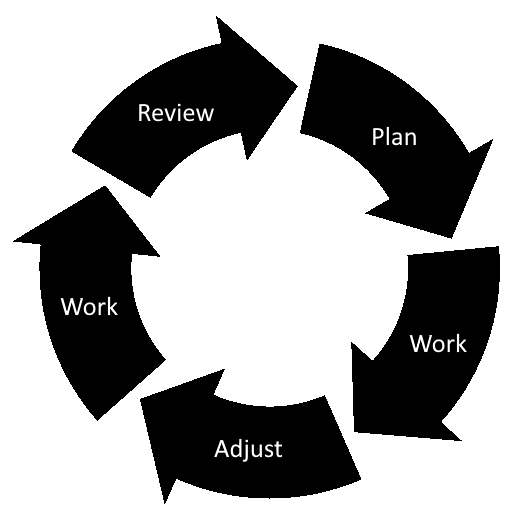
\includegraphics[scale=0.5]{02-Body/Images/WorkIterations.png}
\caption{Illustration of our work iteration}
\label{fig:iterate}
\end{figure}

Once the tasks of the coming week had been decided and assigned, we worked individually, meeting again Wednesday morning for a supervisor meeting, which often took the shape of a short recap of our progress and a discussion with our supervisor, getting a fresh perspective on our solutions and challenges. Following the supervisor meeting we adjusted the planed tasks, taking the new perspective into consideration.

The adjusted tasks were then worked on until the next Monday meeting, resulting in an iterative process as illustrated in figure \ref{fig:iterate}.\\

The tasks for the week was chosen from a "minimal viable progress" perspective. We
considered our progress, and what was the smallest step towards answering the problem
statement. These small steps then became the next tasks. The goal was to ensure that
we always had a working product, and to prevent engaging in massive changes, that
might cost weeks of time if they lead nowhere. \\

By splitting the progress into small steps, we could explore options safe in the
knowledge that we would not spend weeks on a dead end - at least not without some working elements. This only really became relevant in the early stages, where we attempted to write a parser from scratch. When we had no working prototype after the first week, we decided to timebox it one more week, and, as it was not finished, or even near completion, after the timebox, we decided to abandon this path, and to go with the Flex/Bison modules.

